\documentclass[11pt]{article}
\usepackage{enumerate}
\usepackage{fullpage}
\usepackage{fancyhdr}
\usepackage{amsmath, amsfonts, amsthm, amssymb}
\usepackage{graphicx}
\usepackage{wasysym}
\usepackage{bbm}

\setlength{\parindent}{0pt}
\setlength{\parskip}{5pt plus 1pt}
\pagestyle{empty}

%%%%%%%%%%%%%%%%%%%%%%%HEADER%%%%%%%%%%%%%%%%%%%%%%%%%%%%%%
\newcommand{\myname}{Shashank Singh\footnote{sss1@andrew.cmu.edu}
        \footnote{Machine Learning Department \& Department of Statistics}}
\newcommand{\myclass}{10-715 Advanced Introduction to Machine Learning}
\newcommand{\myhwnum}{3}
\newcommand{\duedate}{Wednesday, November 12, 2014}
%%%%%%%%%%%%%%%%%%%%%%%%%%%%%%%%%%%%%%%%%%%%%%%%%%%%%%%%%%%

%%%%%%%%%%%%%%%%%%%%CONTENT MACROS%%%%%%%%%%%%%%%%%%%%%%%%%
\renewcommand{\qed}{\quad \ensuremath{\blacksquare}}
\newcommand{\inv}{^{-1}}
\newcommand{\bv}{\mathbf{v}}
\newcommand{\bx}{\mathbf{x}}
\newcommand{\by}{\mathbf{y}}
\newcommand{\bff}{\mathbf{f}}
\newcommand{\bzero}{\mathbf{0}}
\newcommand{\bxi}{\boldsymbol{\xi}}
\newcommand{\boldeta}{\boldsymbol{\eta}}
\newcommand{\dist}{\operatorname{dist}}
\newcommand{\area}{\operatorname{area}}
\newcommand{\vspan}{\operatorname{span}}
\newcommand{\Gr}{\operatorname{Gr}} % graph of a function
\renewcommand{\sp}{\operatorname{span}} % span of a set
\newcommand{\sminus}{\backslash}
\newcommand{\E}{\mathbb{E}} % expected value
\newcommand{\F}{\mathcal{F}}
\renewcommand{\H}{\mathcal{H}}
\newcommand{\pr}{\mathbb{P}} % probability
\newcommand{\Var}{\operatorname{Var}} % variance
\newcommand{\Cov}{\operatorname{Cov}} % covariance
\newcommand{\tr}{\operatorname{tr}} % trace
\newcommand{\N}{\mathbb{N}} % natural numbers
\newcommand{\Z}{\mathbb{Z}} % integers
\newcommand{\Q}{\mathbb{Q}} % rational numbers
\newcommand{\R}{\mathbb{R}} % real numbers
\newcommand{\A}{\mathcal{A}}
\newcommand{\B}{\mathcal{B}}
\newcommand{\C}{\mathcal{C}} % compact functions
\newcommand{\K}{\mathbb{K}} % underlying field of a linear space
\newcommand{\Ran}{\mathcal{R}} % range of a linear operator
\newcommand{\Nul}{\mathcal{N}} % null-space of a linear operator
\renewcommand{\L}{\mathcal{L}} % bounded linear functions
\newcommand{\pow}[1]{\mathcal{P}\left(#1\right)} % power set of #1
\newcommand{\e}{\varepsilon} % \varepsilon
\newcommand{\wto}{\rightharpoonup} % weak convergence
\newcommand{\wsto}{\stackrel{*}{\rightharpoonup}} % weak-* convergence
\newcommand{\X}{\mathcal{X}}
\newcommand{\Y}{\mathcal{Y}}
\renewcommand{\P}{\mathbb{P}}   % probability
\newcommand{\ind}{\perp\!\!\!\perp} % independent
%%%%%%%%%%%%%%%%%%%%%%%%%%%%%%%%%%%%%%%%%%%%%%%%%%%%%%%%%%%

\begin{document}
\thispagestyle{plain}

{\Large Homework \myhwnum, Problems 1 and 2} \\
Name: \myname \\
\myclass \\
Due: \duedate

\section{Dimensionality Reduction (Samy)}
\subsection{Principal Component Analysis}
\begin{enumerate}
\item We want to maximize $\frac1n \sum_i = 1^n (a_1^T X_i)^2$ subject to
$\|a_1\|_2^2 = 1$. The Lagrangian of this is
\[L(a_1,\lambda)
    = \frac1n \sum_{i = 1}^n (a_1^T X_i)^2 - \lambda(\|a_1\|_2^2 - 1).\]
Thus, stationarity gives
\[0
    = \nabla_{a_1} L(a_1, \lambda)
    = \frac1n \sum_{i = 1}^n 2(a_1^T X_i)X_i - 2\lambda a_1,
\]
which can be re-written as
$n\lambda a_1 = \sum_{i = 1}^n X_iX_i^Ta_1 = X^TXa_1$. Maximizing $\lambda$
tells us that $a_1$ is the first right singular vector of $X$. \qed

\item Now, we are maximizing $\frac1n \sum_{i = 1}^n (a_{k + 1}^T \tilde x_i)^2$
subject to $\|a_{k + 1}\|_2^2 = 1$. For
$\tilde x = [\tilde x_1^T;\cdots;\tilde x_n^T]$, it follows from part 1. that
$a_{k + 1}$ is the first right singular vector of $\tilde x$.

Since singular vectors are orthogonal, the singular vectors of $\tilde x$ are
the same as those of $X$, and the singular values of $\tilde x$ are the
singular values of $X$ with the first $k$ replaced by zero. Hence, $a_{k + 1}$
is the $(k + 1)^{th}$ right singular vector of $X$. \qed
\end{enumerate}
\subsection{Affine Subspace Identification (ASI)}
\begin{enumerate}
\item By construction of $A_2,b_2$, and $Z_2$,
\begin{align*}
\|x_i - A_2Z_{2,i} - b_2\|
 &  = \left\| x_i - A_1C\inv (Z_1C^T + 1d^T)_i - b_1 + A_1C\inv d \right\|  \\
 &  = \left\| x_i - A_1C\inv\left( (Z_1C^T + 1d^T)_i - d \right) - b_1 \right\| \\
 &  = \left\| x_i - A_1C\inv\left( CZ_{1,i} + d_i - d \right) - b_1 \right\|
    = \left\| x_i - A_1Z_{1,i} - b_1 \right\|,
\end{align*}
and it follows that $J(A_2,b_2,Z_2) = J(A_1,b_1,Z_1)$. \qed
\end{enumerate}
\begin{enumerate}
\item Stationarity gives
\begin{align*}
0
    = \nabla_b \sum_{i = 1}^n \|Az_i + b - x_i\|^2
 &  = \sum_{i = 1}^n Az_i + b - x_i,
\end{align*}
which implies
$b = \frac1n \sum_{i = 1}^n x_i - Az_i
    = \frac1n \sum_{i = 1}^n x_i$ (since $\bar{Z} = 0$),
\begin{align*}
0
 &  = \nabla_{z_j} \sum_{i = 1}^n \|Az_i + b - x_i\|^2
        + \sum_{k = 1}^d \lambda_k z_{i,k}
        + \sum_{k = 1}^d \sum_{\ell = 1}^d
                            \mu_{k,\ell} (z_{i,k}z_{i,\ell} - \Psi_{k,\ell}) \\
 &  = A^T(Az_j + b - x_j) + \vec\lambda + 2z_j^T1_d1_d
\end{align*}
for some $\lambda \in \R^d, \mu \in \R^{d \times d}$, and
\begin{align*}
0
    = \nabla_A \sum_{i = 1}^n \|Az_i + b - x_i\|^2
 &  = \sum_{i = 1}^n \nabla_A \|Az_i\|^2 + 2(Az_i)^T(b - x_i) + \|b - x_i\|^2 \\
 &  = \sum_{i = 1}^n 2Az_iz_i^T + 2(b - x_i)z_i^T,
\end{align*}
which implies
\[A
    = \left( \sum_{i = 1}^n (x_i - b)z_i^T \right)
                                \left( \sum_{i = 1}^n z_iz_i^T \right)\inv
    = \left( \sum_{i = 1}^n (x_i - b)z_i^T \right)
                                \left( n \Psi \right)\inv
.\]
Note that, since $b = \bar X$, minimizing $J(A,b,Z)$ is equivalent to
minimizing the Frobenius norm $\|AZ^T - X_c\|_F$ (where $X_c$ denotes the
demeaned version of $X$), under the constraint which is minimized when
$AZ^T = U_dS_dV_d$ is the rank $d$ truncated singular decomposition of $X_c$.
The second constraint can be rewritten as $Z^TZ = n\Psi$, and so
$nA\Psi = AZ^TZ = U_dS_dV_dZ$ and $nA\Psi A^T = nAZ^TZA^T = U_dS_dS_d^TU_d^T$.
I didn't have time to find a closed form for $A$ and $Z$.

\item The $d$ dimensional representation $z_*$ of $x_*$ satisfies
\[z_* = \arg\min_z \|Az_* - x_*\|^2,\]
the usual least squares problem (as in linear regression), whose solution is
\fbox{$z_* = (A^TA)\inv A^Tx_*$.}
\end{enumerate}

\subsection{Factor Analysis (FA)}
\begin{enumerate}
\item Since $z$ and $x|z$ are normally distributed, and the sum and joint
of normally distributed variables are themselves normally distributed, $(z,x)$
has a normal distribution $\mathcal{N}(\mu_{zx},\Sigma)$ on $\R^{D + d}$. Since
$\E[z] = 0$ and $\E[x] = \E[\E[x | z]] = \E[Az + b] = A\E[z] + b = b$,
$\mu_{zx} = (0,b)$. Since $\Cov(z,z) = \Psi$,
\begin{align*}
\Cov(z,x)
    = \E[(z - \E[z])(x - \E[x])^T]
 &  = \E[z(Az + x - Az + b)^T]  \\
 &  = \E[z(Az)^T] + \E[z]\E[x - (Az + b)^T]
    = \E[zz^T]A^T
    = \Psi A^T
\end{align*}
(since $z$ is independent of $x - (Az + b)$). Similarly,
\begin{align*}
\Cov(x,x)
 &  = \E[(x - \E[x])(x - \E[x])^T]
    = \E[(Az + x - (Az + b))(Az + x - (Az + b))^T]  \\
 &  = \E[Az(Az)^T] + 2\E[Az]\E[x - (Az + b)^T] + \E[(x - (Az + b))(x - (Az + b))^T] \\
 &  = A\E[zz^T]A^T + 2A\E[z]\E[x - (Az + b)^T] + \E[(x - (Az + b))(x - (Az + b))^T] \\
 &  = A \Psi A^T + \eta^2 I,
\end{align*}
and so
\[\Sigma =
    \begin{bmatrix}
        \Psi & \Psi A^T \\
        A \Psi^T & A \Psi A^T + \eta^2 I
    \end{bmatrix}.
\]
Consequently, the marginal distribution in $x$ is
$x \sim \mathcal{N}(b, A \Psi A^T + \eta^2 I)$.
Using Fact 1, we can also derive the conditional distribution of $z$ given $x$:
\[z | x
    \sim \mathcal{N} \left(
        \Psi A^T (A \Psi A^T + \eta^2 I) (x - b),
        \Psi - \Psi A^T (A \Psi A^T + \eta^2 I)\inv A \Psi^T
    \right).
\]
\item Since the marginal distribution of the data is
$x \sim \mathcal{N}(b, A \Psi A^T + \eta^2 I)$, the likelihood is
\begin{align*}
L(b, A, \eta)
 &  \propto \prod_{i = 1}^n
        \exp \left( -\frac12 (x - b)^T(A \Psi A^T + \eta^2 I)\inv(X_i - b) \right),
\end{align*}
and hence, for some $C \in \R$, the log-likelihood is
\[\ell(b, A, \eta)
    = C + \sum_{i = 1}^n - \frac12
                        \left\|(A \Psi A^T + \eta^2 I)^{-1/2}(b - X_i)\right\|^2.
\]
Note that, as the inverse of a sum of positive definite matrices,
$A \Psi A^T + \eta^2 I)\inv$ is positive definite, and so $\ell$ is concave in
$b$. Setting the derivative in $b$ to zero gives
\[0
    = \sum_{i = 1}^n (A \Psi A^T + \eta^2 I)^{-1/2} (X_i - b),
\]
which implies $b = \frac{1}{n} \sum_{i = 1}^n X_i$ (since
$(A \Psi A^T + \eta^2 I)^{-1/2}$ is invertible).
\item We lower bound the log-likelihood by
\[\ell(b,A,\eta)
    \geq \sum_{i = 1}^n \E_{z \sim R(z | x)}\left[ \log \frac{p(z, x)}{R(z | x)} \right]
\]
\item
\begin{align*}
\E_{z \sim R(z | x)}\left[ \log \frac{p(z, x)}{R(z | x)} \right]
 &  = \sum_{i = 1}^n \E_{z_i \sim R( \cdot | x_i)}
        \left[ \log p(x_i | z_i, b, A, \eta) + \log p(z_i)
                                                - \log R(z_i | x_i) \right] \\
 &  = \sum_{i = 1}^n \E_{z_i \sim R( \cdot | x_i)}
        \left[ C + \log \left( (2\pi\eta^2)^{-D/2}
            \exp \left( -\frac{\|Az_i + b - x_i\|^2}{2\eta^2} \right) 
                                                            \right) \right] \\
 &  = \sum_{i = 1}^n \E_{z_i \sim R( \cdot | x_i)}
        \left[ C - D\log(\eta) - \frac{\|Az_i + b - x_i\|^2}{2\eta^2} \right]
\end{align*}
where $C$ contains terms not depending on $A$ or $\eta$.
\item Setting the derivative in $\eta$ to zero gives
\begin{align*}
0
 &  = \sum_{i = 1}^n \E_{z_i \sim R( \cdot | x_i)}
        \left[ \frac{d}{d\eta} -D\log(\eta)
                            - \frac{\|Az_i + b - x_i\|^2}{2\eta^2} \right]  \\
 &  = \sum_{i = 1}^n -D/\eta + \E_{z_i \sim R( \cdot | x_i)}
        \left[ \frac{\|Az_i + b - x_i\|^2}{\eta^3} \right].  \\
\end{align*}
Noting $\|Az + b - x\|^2 = \|Az\|^2 + 2(Az)^T(b - x) + \|b - x\|^2$ and solving
for $\eta$ gives
\begin{align*}
\eta
 &  = \frac{1}{nD} \sum_{i = 1}^n \E_{z \sim R( \cdot | x_i)}
                        [\|Az\|^2 + 2(Az)^T(b - x_i) + \|b - x_i\|^2] \\
 &  = \frac{1}{nD} \sum_{i = 1}^n \tr(A \Psi A^T)
    + 2\mu_{z_i|x_i}^T A^T(b - x_i) + \|b - x_i\|^2,
\end{align*}
where $\mu_{z|x} = \E[z | x]$ as computed in part 1., and noting $\E[z] = 0$
and $Az \sim \mathcal{N}(0,A \Psi A^T)$. Setting the derivative in $A$ to zero
gives
\begin{align*}
0
 &  = \nabla_A \sum_{i = 1}^n \E_{z \sim R( \cdot | x_i)}
        \left[ \|Az\|^2 + 2(Az)^T(b - x_i) + \|b - x_i\|^2 \right]  \\
 &  = \sum_{i = 1}^n \E_{z \sim R( \cdot | x_i)}
        \left[ \nabla_A z^TA^TAz + 2z^TA^T(b - x_i) \right] \\
 &  = \sum_{i = 1}^n \E_{z \sim R( \cdot | x_i)}
        \left[ 2Azz^T + 2(b - x_i)z^T \right]    \\
 &  = \sum_{i = 1}^n A\E[zz^T] + \E[z](b - x_i)^T
    = \sum_{i = 1}^n A(\mu_{z_i|x_i}\mu_{z_i|x_i}^T + \Sigma_{z_i|x_i})
        + (b - x_i)\mu_{z_i|x_i}^T,
\end{align*}
where $\Sigma_{z|x} = \Cov[z,z | x]$ as computed in part 1. Solving for $A$
gives
\[A = \left( \sum_{i = 1}^n (x_i - b)\mu_{z_i|x_i}^T \right)
        \left( \sum_{i = 1}^n \mu_{z_i|x_i}\mu_{z_i|x_i}^T + \Sigma_{z_i|x_i} \right) \inv.
\]
\end{enumerate}

\subsection{Experiment}
I wasn't able to get ASI and FA working correctly, but I present the results
for the three PCA variants.

\begin{figure}[h!]
\centering
\quad\;
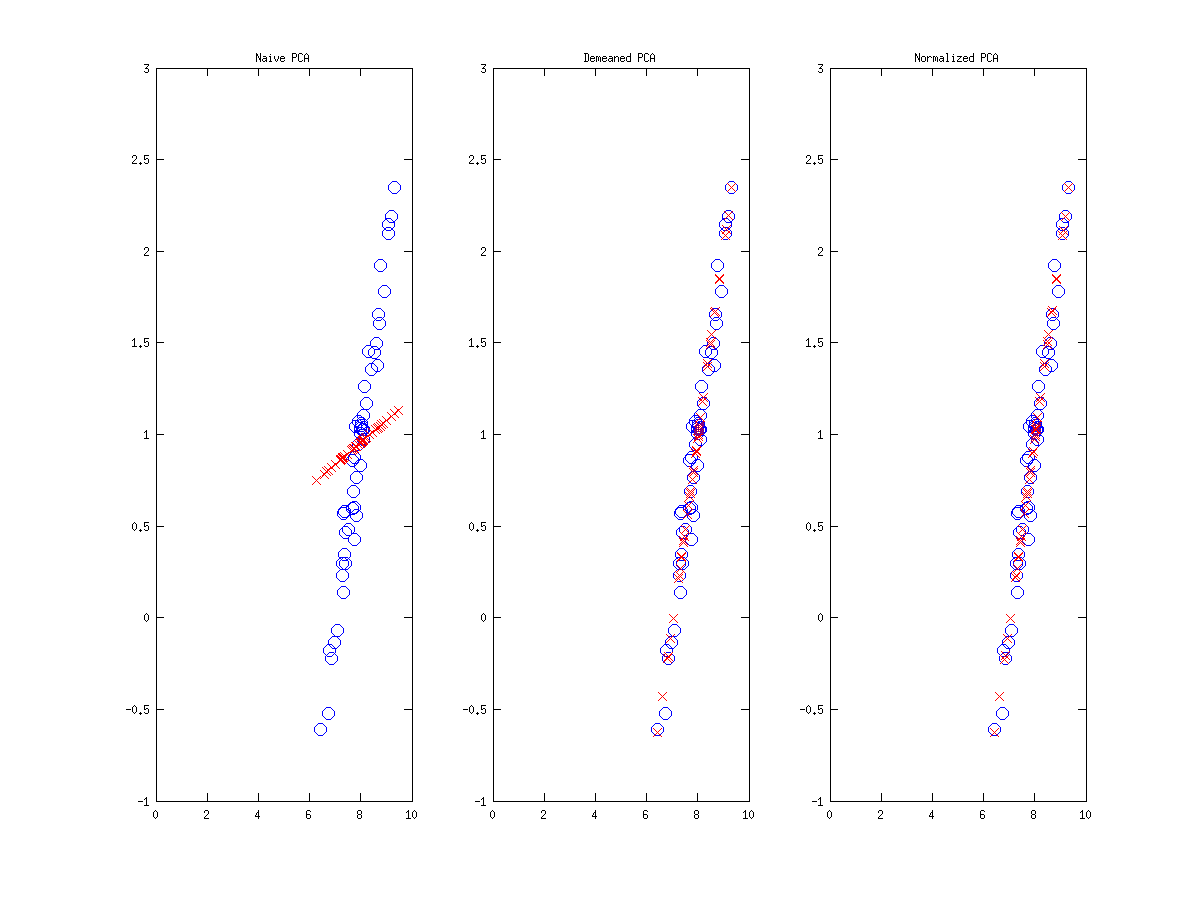
\includegraphics[trim=22mm 0mm 15mm 0mm, clip=true, width=0.6\linewidth]{14results}
\vspace{-12mm}
\caption{$2D$ reconstruction of $1D$ reduced data for all PCA variants.}
\label{fig:14results}
\end{figure}

The reconstruction results for the $2D$ dataset are shown in Figure
\ref{fig:14results}.
The reconstruction errors for the $2D$ dataset were:
\begin{verbatim}
Reconstruction Errors:
Buggy PCA: 0.365284
Demeaned PCA: 0.008448
Normalized PCA: 0.008454
\end{verbatim}
and the reconstruction errors for the $1000D$ dataset were:
\begin{verbatim}
Reconstruction Errors:
Buggy PCA: 29818.420240
Demeaned PCA: 28204.962447
Normalized PCA: 28212.163185
\end{verbatim}

Choice of $d$ for $1000D$ dataset: We first plot the singular values of $X$:
\begin{verbatim}
[~,S,~] = svd(X); svs = diag(S); plot(svs(2:end));
\end{verbatim}
It is fairly clear from the resulting plot (Figure \ref{fig:s_vals}) that first
$31$ singular vectors are the most important, since the first $31$ singular
vectors are all in the $500-900$ range (excepting the first, which is much
bigger), whereas all later singular values are less than $30$.
\begin{figure}[h!]
\centering
\quad\;
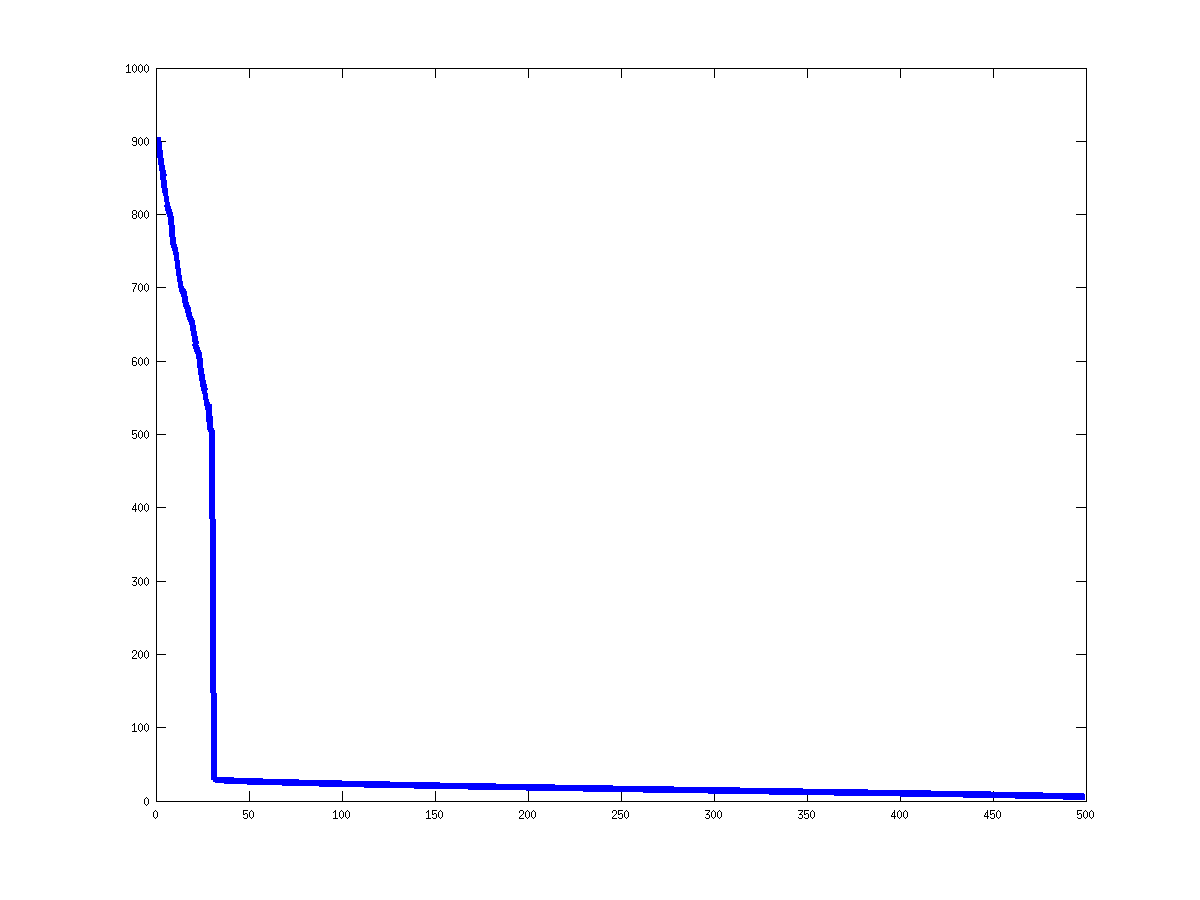
\includegraphics[trim=10mm 0mm 10mm 0mm, clip=true, width=0.6\linewidth]{s_vals}
\vspace{-6mm}
\caption{$2^{nd}$ through $1000^{th}$ singular vectors of data matrix $X$.}
\label{fig:s_vals}
\end{figure}
\vspace{-2mm}
\subsubsection*{Questions}
\begin{enumerate}
\item Buggy PCA projects onto the subspace (through the origin) which
minimizes the reconstruction error. The data lies near an affine subspace, so
reconstruction error is high.
\item We showed in the derivation of ASI that $AZ$ is the rank $d$ truncated
singular value decomposition of a demeaned $X$, which is precisely the
approximation of $X$ used in demeaned PCA. Since the reconstructions are
identical, the errors are as well.
\item This isn't surprising because, by definition, ASI and PCA choose a
representations that minimize reconstruction error of the data, whereas FA
instead maximizes a likelihood and normalized PCA minimizes the reconstruction
error of the normalized data (which, e.g. weighs directions of large variance
less than unnormalized PCA).
\end{enumerate}

%\newpage
\newpage
\subsubsection*{Code}
\begin{verbatim}
function [Z, params, Y] = buggyPrinCompAnalysis(X, d)
  params = 0;
  [~, ~, V] = svd(X);
  PC = V(:,1:d);
  Z = X * PC;
  Y = Z * PC';
end

function [Z, params, Y] = deMeanPrinCompAnalysis(X, d)
  m = mean(X, 1);
  [Z, params, Y] = buggyPrinCompAnalysis(bsxfun(@minus, X, m), d);
  Y = bsxfun(@plus, Y, m);
end

function [Z, params, Y] = normPrinCompAnalysis(X, d)
  m = mean(X, 1);
  X2 = bsxfun(@minus, X, m); % demeaned X
  norms = sqrt(sum(X2.^2,1));
  [Z, params, Y] = buggyPrinCompAnalysis(bsxfun(@rdivide, X2, norms), d);
  Y = bsxfun(@times, Y, norms);
  Y = bsxfun(@plus, Y, m);
end
\end{verbatim}

\section{Some Random Topics (Samy)}
\subsection{K-means Clustering}
\begin{enumerate}
\item 
For $K \in \N$, suppose $\mu_1,\dots,\mu_K$ and $f : \X \to \{1,\dots,K\}$
minimizing $J(\mu_1^K, f; X_1^n)$. Let $\mu_{K + 1} \in \X$, and let
$g : \X \to \{1,\dots,K,K + 1\}$ such that $g(x) = f(x)$ for all $x \in \X$.
Then, $J_K(X_1^n) = J(\mu_1^{K + 1}, g; X_1^n) = J(\mu_1^K, f; X_1^n)$, and
hence $J_K(X_1^n) \leq J_{K + 1}(X_1^n)$. \qed

\item For $i \in \N, j \in \{1,\dots,K\}$, let $\mu_j(i)$ denote the $j^{th}$
centroid and let $f_i$ denote the cluster assignments computed in the $i^{th}$
step of the algorithm. Setting the gradient of the objective in $\mu$ to $0$
shows that
\[\mu_j(i)
    = \frac{1}{n_j} \sum_{k = 1}^n \mathbbm{1}(f_i(X_k) = j) X_k
    = \arg\min_{\mu} \sum_{k = 1}^n
        \mathbbm{1}(f_i(X_\ell) = j) \|X_k - \mu_j(i)\|^2,
\]
so that $\mu_1^K(i) = \arg\min_{\mu_1^K} J(\mu_1^K,f_i;X_1^n)$. By
construction of the $K$-means algorithm,
\[f_i = \arg\min_f J(\mu_1^K(i - 1), f; X_1^n).\]
Hence, $J$ is non-increasing with each iteration. Since there are only finitely
many possible values of $\mu_1^K$ and $f$ (one per partition of $\{1,\dots,n\}$
into $K$ subsets), $J(\mu_1^K(i), f_i; X_1^n)$ is eventually constant and the
algorithm terminates. \qed
\end{enumerate}

\newpage
\subsection{Independent Components Analysis}
\begin{enumerate}
\item See Figure \ref{fig:q23} and code below.
\begin{figure}[h!]
\centering
\quad\;
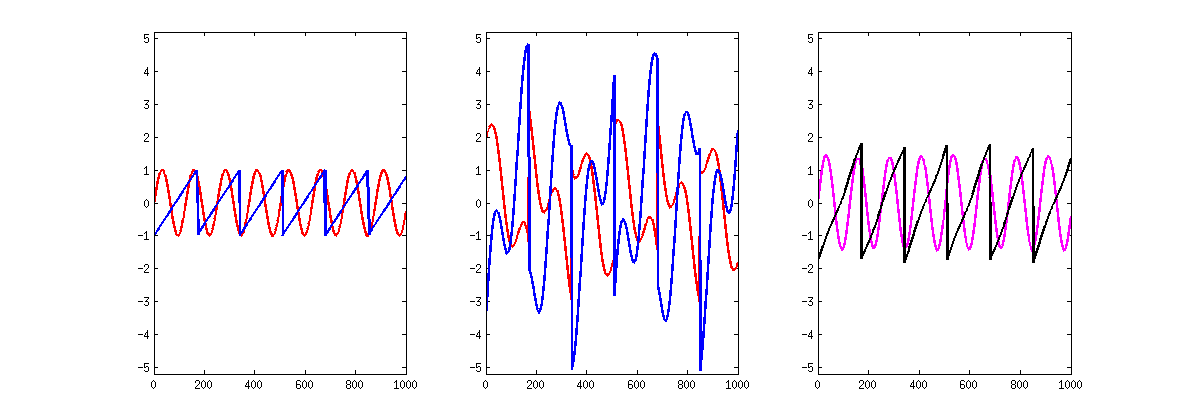
\includegraphics[trim=10mm 0mm 10mm 0mm, clip=true, width=\linewidth]{q23}
\vspace{-6mm}
\caption{Original, mixed, and unmixed signal for question 1 in Section 2.2.}
\label{fig:q23}
\end{figure}
\subsubsection*{Code:}
\begin{verbatim}
N = 1000;
signal1 = sin(linspace(0,50,N));
signal2 = sawtooth(linspace(0,37,N));
subplot(1,3,1); % plot original signals
plot(1:N, signal1, 'r', 1:N, signal2, 'b', 'linewidth', 2); ylim([-5.2 5.2]);

mix1 = signal1 - 2*signal2;
mix2 = 1.73*signal1 + 3.41*signal2;

subplot(1,3,2); % plot mixed signals
plot(1:N, mix1, 'r', 1:N, mix2, 'b', 'linewidth', 2); ylim([-5.2 5.2]);

rec = fastica([mix1; mix2]);
rec1 = rec(1,:); rec2 = rec(2,:);

subplot(1,3,3); % plot unmixed signals
plot(1:N, rec1, 'm', 1:N, rec2, 'k', 'linewidth', 2); ylim([-5.2 5.2]);
\end{verbatim}
\item We are trying determine a matrix factorization $Y = MX$ (where
$Y$ is the input to the algorithm, and $M$ and $X$ are the unknown mixing
matrix and original components, respectively). For any (nonsingular) scaling
(i.e., diagonal) matrix $D$, $Y = MD\inv DX$, and the rows of $DX$ are still
independent, i.e., the input to the algorithm is invariant to scaling the
original components and inversely scaling the mixing matrix. \qed
\end{enumerate}

\newpage
{\Large Homework \myhwnum, Problems 3 and 4} \\
Name: \myname \\
\myclass \\
Due: \duedate

\section{Graphical Models (Veeru)}
\begin{enumerate}
\item
\begin{enumerate}
\item The distribution factors as $P(I,W,G,L) = P(I)P(W)P(G|I,W)P(L|G)$.
\item We need to know $9$ parameters for $P(I)$, $9$ parameters for $P(W)$,
$9 \cdot 10^2 = 900$ parameters for $P(G|I,W)$, and $9 \cdot 10 = 90$
parameters for $P(L|G)$, for a total of $9 + 9 + 900 + 90 = $\fbox{$1008$}
parameters.
\end{enumerate}
\item
\begin{enumerate}
\item No; $I$ and $W$ are related through $G$, which depends on $L$, e.g., a
student who did little work and received an $A$ was likely very intelligent.
\item No; $I$ and $G$ are directly connected.
\item Yes; $L$ depends only on $G$.
\item No; $G$ depends on $L$ not through $W$; e.g., if $L$ is a function of
$G$.
\end{enumerate}
\item
\begin{enumerate}
\item We first compute the probabilities of $G = 1$ and $G = 2$:
\begin{align*}
P(G = 1)
 &  = P(G = 1 | I = 0, W = 0)P(I = 0)P(W = 0)   \\
 &  + P(G = 1 | I = 0, W = 1)P(I = 0)P(W = 1)   \\
 &  + P(G = 1 | I = 1, W = 0)P(I = 1)P(W = 0)   \\
 &  + P(G = 1 | I = 1, W = 1)P(I = 1)P(W = 1)   \\
 &  = (0.1)(0.3)(0.2)
    + (0.6)(0.3)(0.8)
    + (0.7)(0.7)(0.2)
    + (0.1)(0.7)(0.8)
    = 0.304.
\end{align*}
Since $P(G = 2 | I = 0, W = 0) = 0$,
\begin{align*}
P(G = 1)
 &  + P(G = 2 | I = 0, W = 1)P(I = 0)P(W = 1)   \\
 &  + P(G = 2 | I = 1, W = 0)P(I = 1)P(W = 0)   \\
 &  + P(G = 2 | I = 1, W = 1)P(I = 1)P(W = 1)   \\
 &  = (0.3)(0.3)(0.8)
    + (0.2)(0.7)(0.2)
    + (0.9)(0.7)(0.8)
    = 0.604.
\end{align*}
Since $P(L = 1 | G = 0) = 0$, the probability of $L = 1$ is
\begin{align*}
P(L = 1)
 &  = P(L = 1 | G = 1) P(G = 1) + P(L = 1 | G = 2) P(G = 2) \\
 &  = (0.3)(0.304) + (0.8)(0.604)
    = \mbox{\fbox{$0.5744$.}}
\end{align*}
\item Since $P(L = 1 | G = 0) = 0$, the probability of $L = 1$ given $I = 1$
and $W = 0$ is
\begin{align*}
P(L = 1 | I = 1, W = 0)
 &  = P(L = 1 | G = 1) P(G = 1 | I = 1, W = 0)  \\
 &  + P(L = 1 | G = 2) P(G = 2 | I = 1, W = 0)  \\
 &  = (0.3)(0.7) + (0.8)(0.2)
    = \mbox{\fbox{$0.37$.}}
\end{align*}
\end{enumerate}
\item
\begin{enumerate}
\item The probability of this sequence is approximately
$6.1939 \times 10^{-5}$.
\item The most likely sequence is $2,2,2,2,2,1,1,1,1,1,1,1$.
\end{enumerate}
\end{enumerate}
Code for 4(a) and 4(b) is included below.
\subsubsection*{Code}
\begin{verbatim}
T = [0.7 0.2 0.1; 0.2 0.7 0.1; 0.1 0.3 0.6];
P = [0.9 0.1 0 0; 0.8 0.1 0.1 0; 0.5 0.3 0.1 0.1];
data = min(3,[1 5 0 1 1 0 0 0 0 0 0 0]);

[seq p_tot] = MLE_seq(T, P, data)

function [seq p_tot] = MLE_seq(T, P, data)

  n = length(data);
  k = size(T,1);
  seq = zeros(1,n); % most likely sequence
  l = -Inf; % log-likelihood of seq
  p_tot = 0; % probability of data

  for i=0:(k^n - 1) % for each possible sequence
    seq_new = (dec2base(i, k, ceil(log(k^n)/log(k)) - 1) - '0') + 1;
    l_new = 0; % log-likelihood of new_seq
    for j=1:(n - 1) % for each transition
      l_new = l_new + log(T(seq_new(j), seq_new(j + 1)));
    end
    for j=1:n % for each observation
      l_new = l_new + log(P(seq_new(j), data(j) + 1));
    end

    p_tot = p_tot + exp(l_new);

    if l_new > l
      seq = seq_new - 1;
      l = l_new;
    end
  end
end
\end{verbatim}


\section{Markov Chain Monte Carlo (Veeru)}
\subsection{Markov Chain properties}
\begin{enumerate}
\item Recall first that $T$ and $T^T$ have the same eigenvalues, since
\[\det(A^T - \lambda I)
    = \det((A^T - \lambda I)^T)
    = \det(A - \lambda I),
\]
and $\lambda$ is an eigenvalue if and only if the above determinant is $0$. For
$i \in [n]$ since $j \mapsto T_{ij}$ is the probability density function of
transitions from state $i$, $\sum_{j = 1} T_{ij} = 1$, and so, if
$\mathbbm{1}_n \in \R^n$ is the vector of all ones, then
$\mathbbm{1}_n = T \mathbbm{1}_n$. Thus, $1$ is an eigenvalue of $T$, and hence
of $T^T$. \qed
\item For
\[v_1 =
    \begin{bmatrix}
        0 & 7/6 & 0 & 1
    \end{bmatrix}
    \quad \mbox{ and } \quad
v_2 =
    \begin{bmatrix}
        4/7 & 0 & 1 & 0
    \end{bmatrix},
\]
$v_1T = v_1$ and $v_2T = v_2$ (i.e., $v_1/\|v_1\|_1$ and $v_2/\|v_2\|_1$ both
encode stationary distributions). Intuitively, this reflects the fact that the
Markov chain is reducible. \qed
\item Consider a $2$-state Markov chain with transition matrix and initial
distribution
\[\mbox{\fbox{$\displaystyle
T =
    \begin{bmatrix}
        0 & 1 \\
        1 & 0
    \end{bmatrix}
    \quad \mbox{ and } \quad
p_0 =
    \begin{bmatrix}
        1 & 0
    \end{bmatrix}$.}}
\]
Then, $p_0T^n = p_0$ when $n$ is even, and $p_0T^n = [0 \quad 1]$ when $n$ is
odd, so that $p_0T^n$ does not converge. This occurs because the Markov chain
is periodic.
\end{enumerate}

\subsection{Detailed balance property}
\begin{enumerate}
\item If $\pi$ denotes the target distribution and $T$ denotes the transition
probability, then for any states $x,x'$
\[T(x'|x)
    = g(x'|x) A(x'|x)
    = g(x'|x) \min\left\{ 1, \frac{\pi(x')g(x|x')}{\pi(x)g(x'|x)} \right\}.
\]
where $g$ is the proposal distribution and $A$ is the acceptance distribution.
Since $\pi$ and $g$ are positive, for any states $x,x'$,
\begin{align*}
\pi(x)T(x'|x)
 &  = \pi(x) g(x'|x) \min\left\{ 1, \frac{\pi(x')g(x|x')}{\pi(x)g(x'|x)} \right\}
    = \min\left\{ \pi(x) g(x'|x), \pi(x')g(x|x') \right\}   \\
 &  = \pi(x')g(x|x') \min\left\{ \frac{\pi(x) g(x'|x)}{\pi(x')g(x|x')}, 1 \right\}
    = \pi(x')T(x|x'),
\end{align*}
which is the detailed balance property. \qed
\item Suppose a distribution $\pi$ over the states and a transition matrix $T$
statisfy detailed balance (i.e., $\pi(x)T(x'|x) = \pi(x')T(x|x')$ for all
states $x,x'$). Then, summing over $x'$ on both sides gives
\[\pi(x) = \sum_{x'} \pi(x')T(x|x'),\]
since $T$ is stochastic. Rewriting this vectorially, $\pi = \pi T$, and so
$\pi$ is stationary. \qed
\end{enumerate}

\newpage
\subsection{Experiments}
\begin{enumerate}
\item
\begin{enumerate}
\item The means are: $4.9712, -5.0576, 4.9554, -5.1235, 5.0784$, and $-5.1124$,
which differ substantially from the true population mean of $0$. From Figure
\ref{fig:431a}, it is clear that the sampler is getting ``stuck'' in the two
modes ($-5$ and $5$) of the target distribution.
\begin{figure}[h!]
\centering
\quad\;
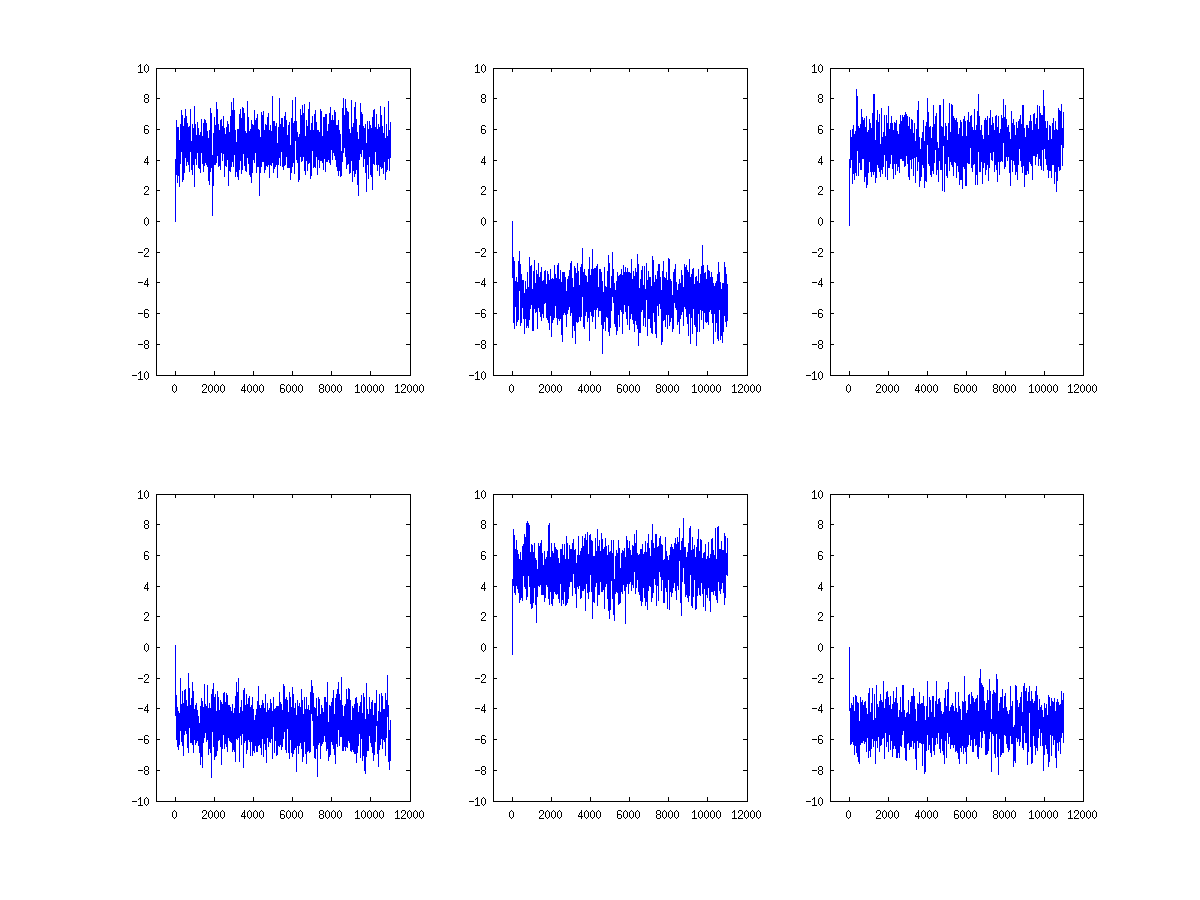
\includegraphics[trim=18mm 0mm 18mm 0mm, clip=true, width=\linewidth]{431a}
\vspace{-6mm}
\caption{Plots of Metropolis-Hastings samples (including burnin samples) for
each of $6$ trials.}
\label{fig:431a}
\end{figure}
\item The means are now $-0.1101, 0.1731, -0.6260, 0.8826, 0.0223$, and
$0.7333$, much closer to the true population mean of $0$. This larger $\sigma$
is better because it allows the sampler to jump between the two modes of the
target distribution.
\item The average of $50$ sample means is $-0.7939$.
\end{enumerate}
Code for Problems 1(a)-(c) of Section 4.3 is included below:
\subsubsection*{Code}
\begin{verbatim}
b = 10^4; % number of burnin samples
n = 10^3; % number of mixed samples
sigma = 0.5; % standard deviation of proposal distribution; also tried 5
Q = @(x_star,x) normpdf(x_star, x, sigma); % proposal density
x0 = 0; % initial x
m = 6; % number of repetitions; also tried 50
mu = 5; % mean of target distribution
pi = @(x) exp(-(x - mu)^2/2) + exp(-(x + mu)^2/2); % target density

means = zeros(m,1);

for rep = 1:m

  samples = zeros(n + b, 1);
  samples(1) = x0;

  for sample = 2:(n + b)
    u = unifrnd(0,1);
    x = samples(sample - 1); % previous sample
    x_star = normrnd(samples(sample - 1),sigma); % sample from proposal

    if u < min(1, pi(x_star)*Q(x, x_star)/(pi(x)*Q(x_star, x)))
      samples(sample) = x_star;
    else
      samples(sample) = x;
    end
  end
  means(rep) = mean(samples(( b + 1):end)); % mean of mixed samples
end
\end{verbatim}
\newpage
\item
\begin{enumerate}
\item By Bayes' Rule,
\begin{align*}
p(z_i = k | x, z_{-i}, \mu)
 &  \propto p(x_i | z_i = k,x_{-i},z_{-i},\mu) p(z_i = k | x_{-i},z_{-i},\mu)\\
 &  = p(x_i | z_i = k,\mu_k) p(z_i = k),
\end{align*}
since $z_i$ is independent of $x_{-i}, z_{-i}$, and $\mu$, and
$x_i$ is conditionally independent of $x_{-i}, z_{-i}$, and $\mu_{-i}$.
Similarly, applying Bayes' Rule again,
\begin{align*}
p(\mu_k = u | x,z,\mu_{-k})
 &  \propto p(x | \mu_k = u,z,\mu_{-k})p(\mu_k = u | z,\mu_{-k})    \\
 &  = p(\mu_k = u | z,\mu_{-k}) \prod_{i = 1}^n p(x_i | \mu_k = u,z,\mu_{-k})\\
 &  = p(\mu_k = u) \prod_{\{i : z_i = k\}} p(x_i | \mu_k = u,z_i = k),
\end{align*}
since (for $i \neq j$) $x_i$ and $x_j$ are conditionally independent given
$\mu$ and $z$, and since $\mu_k$ is independent of $z$ and $\mu_{-k}$, and
$x_i$ is conditionally independent of $\mu_k$ given $z_i \neq k$, and $x_i$ is
conditionally independent of $z_{-k}$ and $\mu_{-k}$ given $z_i = k$. \qed

Note that we can easily resample our estimates of $\mu_1,\dots,\mu_k$ because
our normal prior is conjugate to the normal distribution of the data.

\item The final clustering is shown in Figure \ref{fig:432b}, and code
is included below.
\begin{figure}[h!]
\centering
\quad\;
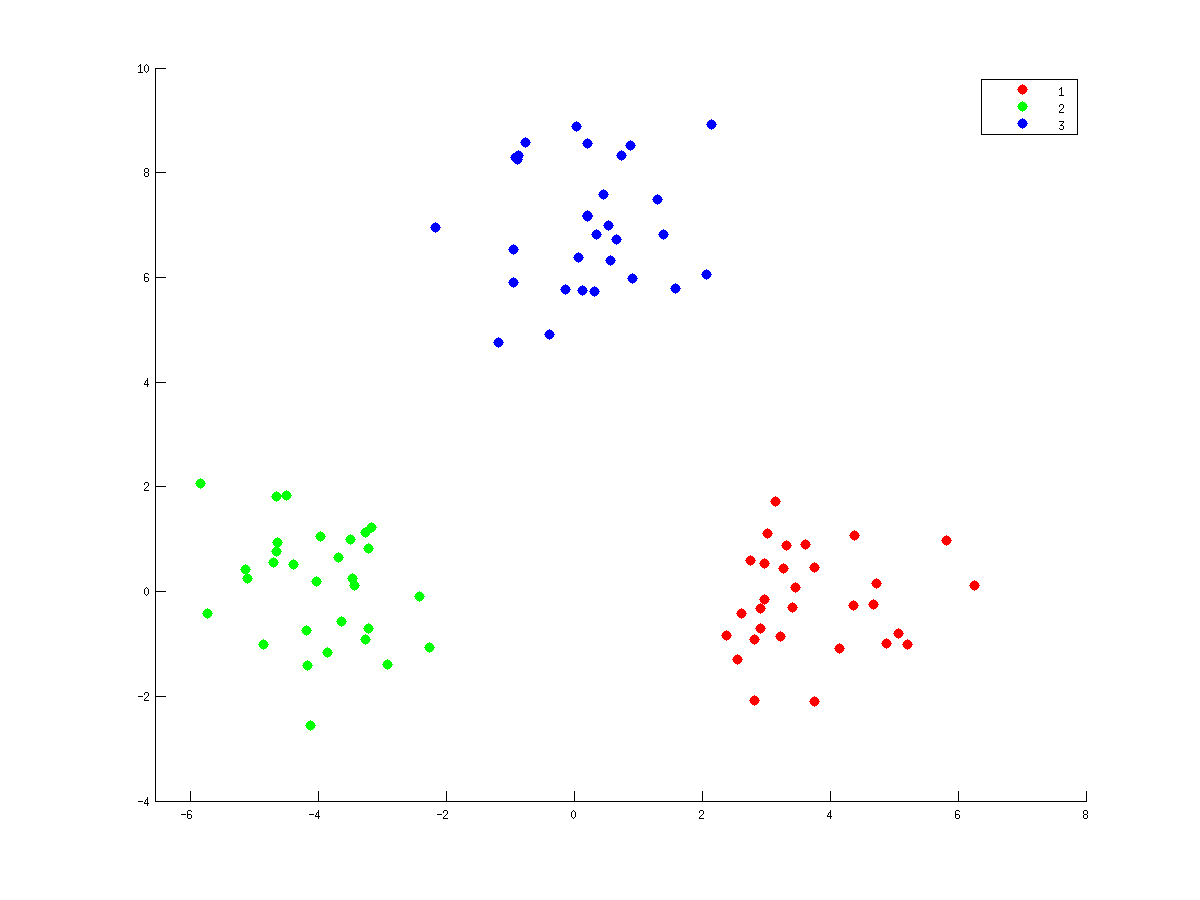
\includegraphics[trim=18mm 0mm 18mm 0mm, clip=true, width=0.65\linewidth]{432b}
\vspace{-6mm}
\caption{Cluster assignments of $90$ data points ($30$ from each cluster).}
\label{fig:432b}
\end{figure}
\end{enumerate}
\end{enumerate}
\subsubsection*{Code}
\begin{verbatim}
n_iters = 5001; % number of Gibbs sampling iterations
n = 30; % number of samples per cluster
true_mus = [-4 0; 4 0; 0 7]; % true cluster means
sigma = 1; % cluster standard deviations
[k d] = size(true_mus); % number of clusters and dimension of data
N = n*k; % total number of samples

Xs = zeros(0, d);
for cluster = 1:k % generate data from each cluster
  Xs = [Xs; normrnd(repmat(true_mus(cluster, :), n, 1), sigma, n, d)];
end

Zs = randi(k, N, 1); % initial (uniformly random) cluster assignments
Mus = mvnrnd(zeros(d, 1), eye(d), k); % initial random cluster means

for iter = 1:n_iters

  for sample = 1:N % resample cluster labels for each sample
    for cluster = 1:k % compute conditional probability given each cluster
      w(cluster) = mvnpdf(Xs(sample, :), Mus(cluster, :));
    end
    % sample cluster label by weight w
    Zs(sample) = sum(rand >= cumsum(w./sum(w))) + 1;
  end

  for cluster = 1:k % resample cluster means for each cluster
    clust_Xs_mean = mean(Xs(Zs &=&  cluster, :), 1);
    n_clust = sum(Zs &=&  cluster);
    sd = 1/(n_clust + 1);
    Mus(cluster, :) = mvnrnd(clust_Xs_mean*n_clust*sd, eye(d)*sd);
  end
end
\end{verbatim}
\end{document}
